\subsection{Semantics}
Let $Q$ be a quantifier, its quantification function $Q : \mathcal{F}(S) \rightarrow [0,1]$. According to the corresponding relation between fuzzy set and Fuzzy Logic, $\mathcal{F}(U)$ equivalent to the set of all interpretations of fuzzy atom. Suppose $p(t_1,...,t_n)$ is an fuzzy atom, and its interpretation is $I$. The semantics of $Q(p(t_1,...,t_n))$ is that quantification function $Q$ assigns a value in $[0,1]$ to the interpretation $I$ of atom $p(t_1,...,t_n)$. As seen it is still defined in second order. In order to define quantification in first order fuzzy predicate, for a quantifier $Q$ and a fuzzy predicate $p$, we generate a new quantifier $Q_p$, which means, $Q_p$ only works on fuzzy predicate $p$. Then the semantics of $Q(p(t_1,...,t_n))$ is that $Q_p$ assigns a value $[0,1]$ to the result from interpretation of $p$, which is $[0,1]$. We formalized it as follows.

\subsubsection{Declarative semantics}
\label{sec:DeclativeSemanticQuantification}
Let \textit{valuation} be $\sigma : V \rightarrow \mathbb{HU}$, and the corresponding 
\textit{extension valuation} be $\hat{\sigma}: \textbf{TB}_{\Pi,\Sigma,V} \rightarrow \mathbb{HB}$,
$\mathcal{I}$ be the \textit{interpretation} $\mathbb{HB} \rightarrow \mathbb{T}$ and $Q_p$ be function $[0,1] \rightarrow [0,1]$, $p/n$ be a arbitrary predicate with arity $n$. 

For a quantifier declaration, its model is an interpretation $\mathcal{I}$, which satisfies,
\[\mathcal{I},\sigma \models Q(p(t_1,...,t_n)) \leftarrow v\] \textbf{iff} $\hat{\sigma}(p(t_1,...,t_n))$ is \textit{well\_typed} and $Q_p(\mathcal{I}(\hat{\sigma}(p(t_1,...,t_n)))) \succeq v$.

\[\mathcal{I} \models Q(p(\vec{t_i})) \leftarrow v\] \textbf{iff} for all \textit{valuation} $\sigma$ which makes $\hat{\sigma}(p(\vec{t_i}))$ \textit{well\_typed}, $Q_p(\mathcal{I}(\hat{\sigma}(p(\vec{t_i})))) \succeq v$.

\subsubsection{Operational semantics}
\label{sec:OperationalSemanticQuantification}

There are two steps taken when evaluate the statement or query $Q(p(t_1,...,t_n))$. The first is generating new quantifier according to $Q$ and $p$, and the second is finalizing the value.

\begin{itemize}
\item Generating
\begin{figure}[h!]
\begin{center}
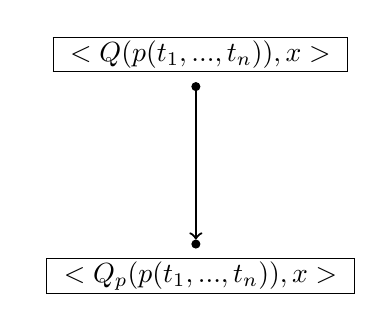
\begin{tikzpicture}[yscale=-1,
place/.style={circle,draw=black, fill=black, inner sep=0pt, 
              minimum size=1mm}]

\node[place] (1st) at (0, 0) [label=above: {
             \begin{tabular}{|c|}
               \hline
              	$<Q(p(t_1,...,t_n)),x>$\\
               \hline
             \end{tabular} }] {};

\node[place] (2nd) at (0, 2) [label=below: {
             \begin{tabular}{|c|}
               \hline
               $<Q_p(p(t_1,...,t_n)),x>$ \\
               \hline
             \end{tabular} }
] {};
        
	\draw[->, thick] (1st) -- (2nd);


\end{tikzpicture}
\end{center}
\caption{Generate new quantifier $Q_p$}
\label{fig:Generating}   
\end{figure}
\item Finalizing
\begin{figure}[h!]
\begin{center}
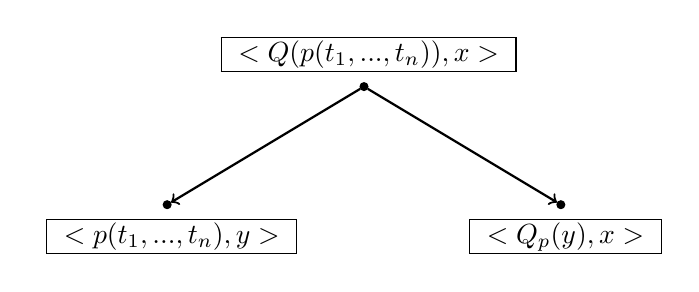
\begin{tikzpicture}[yscale=-1,
place/.style={circle,draw=black, fill=black, inner sep=0pt, 
              minimum size=1mm}]

  \node[place] (1st) at (2.5, 0) [label=above: { 
             \begin{tabular}{|l|}
               \hline
               $<Q(p(t_1,...,t_n)),x>$\\
               \hline
             \end{tabular} }
] {};
	\node[place] (2nd) at (0, 1.5) [label=below: {
              \begin{tabular}{|l|}
                \hline
                 $<p(t_1,...,t_n),y>$ \\
                \hline
              \end{tabular} }
] {};

        \node[place] (3rd) at (5, 1.5) [label=below: {
              \begin{tabular}{|l|}
               \hline
              $<Q_p(y),x>$ \\
               \hline
              \end{tabular} }
] {}; 

	\draw[->, thick] (1st) -- (2nd);
        \draw[->, thick] (1st) -- (3rd);
\end{tikzpicture}
\end{center}
\caption{Finalize the value}
\label{fig:Finalizing}   
\end{figure}
\end{itemize}

\begin{ex}
Suppose that \textbf{friendly} is a binary predicate, and \textbf{quite} is a fuzzy quantifier. The fact is 
$friendly(Freddy,Irene)=0.7$, and $quite_{friendly}$ is a function $[0,1] \rightarrow [0,1]$.
\[  quite_{friendly}(x) = \left\{ 
  \begin{array}{l l}
    0 & \quad \text{if 0 $0 \leq x < 0.4$}\\
    7/8*x & \quad \text{if $0.4 \leq x < 0.8$}\\
    x & \quad \text{if $0.8 \leq x \leq 1.0$}\\
  \end{array} \right.
\]
The query ``Are Freddy and Irene quite friendly with each other ?" is represented as $<quite(friendly(Freddy, Irene)),V>$. And the evaluation of this query works by taking two step generating and finalizing.
\begin{figure}[h!]
\begin{center}
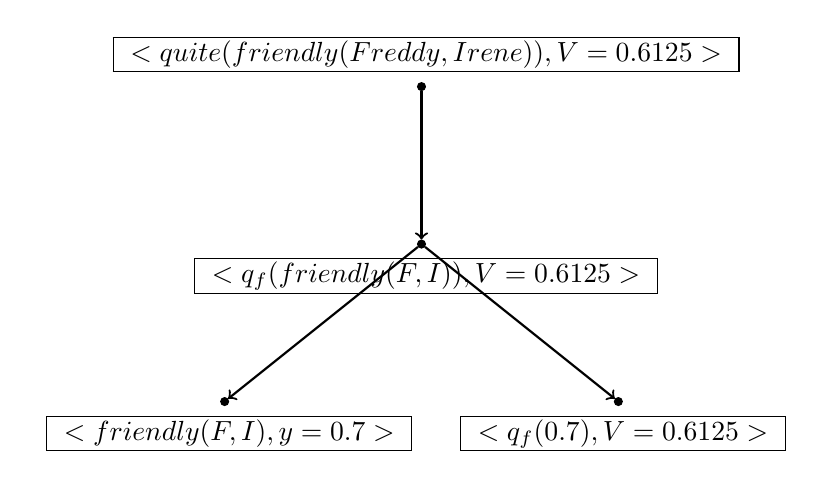
\begin{tikzpicture}[yscale=-1,
place/.style={circle,draw=black, fill=black, inner sep=0pt, 
              minimum size=1mm}]

\node[place] (1st) at (2.5, 0) [label=above: {
             \begin{tabular}{|c|}
               \hline
              	$<quite(friendly(Freddy,Irene)), V=0.6125>$\\
               \hline
             \end{tabular} }] {};

\node[place] (2nd) at (2.5, 2) [label=below: {
             \begin{tabular}{|c|}
               \hline
               $<q_{f}(friendly(F,I)),V=0.6125>$ \\
               \hline
             \end{tabular} }
] {};
        
	
\node[place] (3rd) at (0, 4) [label=below: {
              \begin{tabular}{|c|}
                \hline
                 $<friendly(F,I), y=0.7>$ \\
                \hline
              \end{tabular} }
] {};

        \node[place] (4th) at (5, 4) [label=below: {
              \begin{tabular}{|c|}
               \hline
              $<q_{f}(0.7), V=0.6125>$ \\
               \hline
              \end{tabular} }
] {}; 

\draw[->, thick] (1st) -- (2nd);
\draw[->, thick] (2nd) -- (3rd);
\draw[->, thick] (2nd) -- (4th);

\end{tikzpicture}
\end{center}
\caption{Example of evaluating $<quite(friendly(Freddy,Irene)),V>$}
\label{fig:QuiteFriendly}   
\end{figure}
\end{ex}

